% !TeX root = ../thesis.tex
\section{Performance explorations}
\subsection{Memory}
Shared parameters.
Shared temporary arrays - mention gf820 impact.
Constant memory (h variable is currently identical over all plans, though it doesn't have to be... it's the same over all threads anyway)
Test occupancy?

\subsection{Expression reduction}
Talk more about optimizer method -> also try to remove unused method declarations, though it's unlikely to help

\subsection{Artificial Collective Spouse Pension}
The artificial collective spouse pension (``grundform 820'' in Danish) is a pension in which upon the death of the ensured, the spouse if one such exists, receives a life annuity that is potentially deferred.

\subsubsection{Traditional method of computation}
It is traditionally calculated as a 3-tier process.

The \emph{outer model} can be seen as a 2-state (active-dead) Markov-model where the transition cost to the death state is the \emph{middle model}, solved from 120 minus the age of the ensured to 0.
The \emph{middle model} can be seen as another 2-state Markov-model, but rather than using Thiele's equation it calculates $-gp(tau) \cdot h(eta, tau) \cdot Inner(eta, k, t)$ where $gp$ is the marriage-probability of a $tau$-aged individual and $h$ is the probability that a $tau$-aged individual is married to an $eta$-aged individual given that the first individual is married.
This is solved from 120 to 1. The middle model can also be solved using numerical integration.
The \emph{inner model} is another 2-state Markov-model with benefit paid being $indicator(s >= k)$ (indicator returns 1 if true, otherwise zero) and transition intensity being the spouse death mortality probability, solved from 120 minus $eta$ to 0.

It is a fairly complex method of computation as is also apparent in its runtime - up to two and a half minutes on the CPU.
While it can be run on the GPU, it is not particularly suited for it as there is a lot of code branching making threads finish at very different times making them harder to execute in parallel.

\subsubsection{Parallelized method of computation}
An alternative approach was suggested by .... using a single-tier approach.
The Markov-model contains the active state for the insured, 125 intermediary states signifying death of the insured when married to a spouse of an age difference from -62 to 62 and a final state signifying either death of the spouse or death of the ensured as depicted in figure \ref{fig:gf820}.

\begin{figure}[h!]\centering
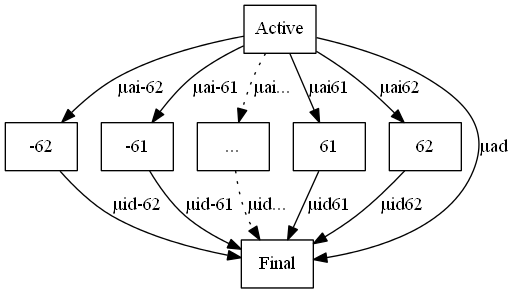
\includegraphics[scale=0.5]{gf820.png}
\caption{Markov-model for the parallelized GF820 Artificial Collective Spouse Pension plan.\label{fig:gf820}}
\end{figure}

The transition probability to one of the intermediary states is the mortality intensity for the ensured at time $t + age$ times the marriage probability of a $t + age$ is married to a $t + age + diff$ year old where $diff$ is the number of the state.
The ensured to final state probability is the mortality intensity of the ensured at time $t + age$ times 1 minus the marriage probability at time $t + age$.
The intermediary to final state probability is simply the mortality intensity of the spouse (assuming the sexuality of the ensured does not change) at age $t + age + diff$.

This does potentially lead to a lot of cases where the ensured will either be married to someone yet to be born or someone significantly older than the oldest person alive today, which is a problem particularly for the Gompertz-Makeham mortality intensity methods. 


Talk about Alea.cuBase issues - expression tree depth and local memory usage (neither worked), talk about current results - broken as fuck.
